\lesson{Preprocessing, Compiler, Assembler, Linker}

In der letzten Lektion habt ihr bereits das erste mal ein Programm kompiliert,
d.h. ihr habt eine für Menschen lesbare Datei in eine für Computer lesbare Datei
übersetzt. Jetzt wollen wir uns etwas genauer anschauen was dabei eigentlich passiert.
Ihr müsst dabei jetzt nicht jedes Detail vestehen, aber es ist praktisch zu
wissen, wie der Compile Vorgang funktioniert um manche Fehlermeldungen zu verstehen.

In Lektion 1 haben wir vereinfacht dargestellt, dass der Compiler eine
Quelltextdatei mit der Endung \texttt{.cpp} nimmt und daraus direkt eine
ausführbare Datei erstellt. Die Schritte, die hier eigentlich in einem Befehl
durchgeführt werden, aber zu trennen sind, sind das \emph{Preprocessing}, das \emph{Kompilieren}, das
\emph{Assemblieren} und das \emph{Linken}.

Beim Preprocessing werden alle \texttt{\#include}-Anweisungen aufgelöst.
Das ist der erste Schritt, der passiert, wenn wir \texttt{g++}
aufrufen. Das Ergebnis des Preprocessings ist ein erweitertes\Cpp-Programm, das nur noch die
\Cpp-Features enthält, die wir auch wirklich benutzen. Das ist der Grund, warum wir
in den bisherigen Lektionen immer \texttt{g++ -o helloworld helloworld.cpp} benutzt haben,
obwohl wir in \texttt{helloworld.cpp} auch \texttt{\#include <iostream>} stehen haben
-- der Compiler hat das schon für uns erledigt.

Das Kompilieren übersetzt unseren erweiterten \Cpp-Code in eine Zwischenform, so genannten
\emph{Assembler}. In Lektion 1 haben wir den Maschinencode angesprochen, in der
Befehle und Parameter an Befehle in 1en und 0en dargestellt werden. Assembler
ist quasi die nächst höhere Evolutionsstufe -- statt die Befehle binär zu
kodieren, gibt es für jeden Befehl ein so genanten \emph{mnemonic}, also ein
merkbares kurzes Wort. Ein Befehl ist allerdings deutlich weniger mächtig, als
z.B. eine Anweisung in \Cpp. Früher wurden ganze Betriebssysteme in Assembler
geschrieben, da es einfach nichts Besseres gab, heutzutage ist Assembler bis
auf die exotischsten Anwendungsfelder eigentlich ausgestorben, da es viel zu
anstrengend und Fehleranfällig ist. Der Compiler tut aber noch mehr, als
einfach nur in diese Zwischensprache zu übersetzen -- er führt auch
\emph{Optimierungen} durch, d.h. er sortiert Anweisungen um, damit der Code
schneller läuft, aber das Gleiche tut. Dieser Prozess ist sehr umständlich,
aber heutige Compiler sind tatsächlich so gut im Optimieren, dass sie meistens
deutlich schnelleren Code erzeugen, als ein Mensch es je könnte.

Der nächste Schritt ist dann das Assemblieren. Das übersetzt den Assembler des
ersten Schrittes tatsächlich in Maschinensprache (genauer: In ein Dateiformat,
welches ELF heißt, welches dann die Maschinensprache plus einiger
Meta-Informationen enthält). Der Assembler erzeugt so genannte
\emph{Objectfiles}, die meistens die Endung \texttt{.o} haben (und im
ELF-Format sind). Ein Objectfile enthält dann mehrere Funktionen (in
Maschinencode) und Variablen, die es \emph{exportieren} kann, d.h. Funktionen
anderer Objectfiles die dagegen (im nächsten Schritt) gelinkt werden, können
diese Variablen und Funktionen sehen. Der Vorteil, diesen Schritt vom
vorhergehenden zu trennen ist, dass wir wenn wir wollen auch nur kompilieren
können und den resultierenden Assembler betrachten -- das kann uns helfen,
Engpässe in unserem Code, an denen der Compiler nicht hinreichend gut optimiert
zu erkennen und möglicherweise zu verbessern. z.B. in der Spielentwicklung ist
sehr schnell laufender Code wichtig.

Der letzte Schritt ist das Linken. Hier werden mehrere Objectfiles genommen und
miteinander verbunden, zu einer ausführbaren Datei. Wenn in einer der
Objectfiles eine \texttt{main}-Funktion existiert, wird diese als
Eintrittspunkt für das Programm genommen, sonst gibt es einen
\emph{Linkerfehler}. Ein Linkerfehler tritt auch auf, wenn wir versuchen, eine
Funktion zu verwenden, die es nicht gibt (z.B. indem wir Funktionen aus einem
Headerfile benutzen ohne das Header-File mit \texttt{\#include} auch tatsächlich einzubinden).
Linkerfehler deuten also darauf hin, dass wir vergessen haben, alle
relevanten Dateien auf der Kommandozeile anzugeben, oder dass eine
\texttt{main}-Funktion fehlt, oder dass wir in mehren Dateien eine Funktion
gleichen Namens haben, oder\dots

Wenn ihr das Programm aus der letzten Lektion kompiliert passiert im Prinzip also
folgendes:

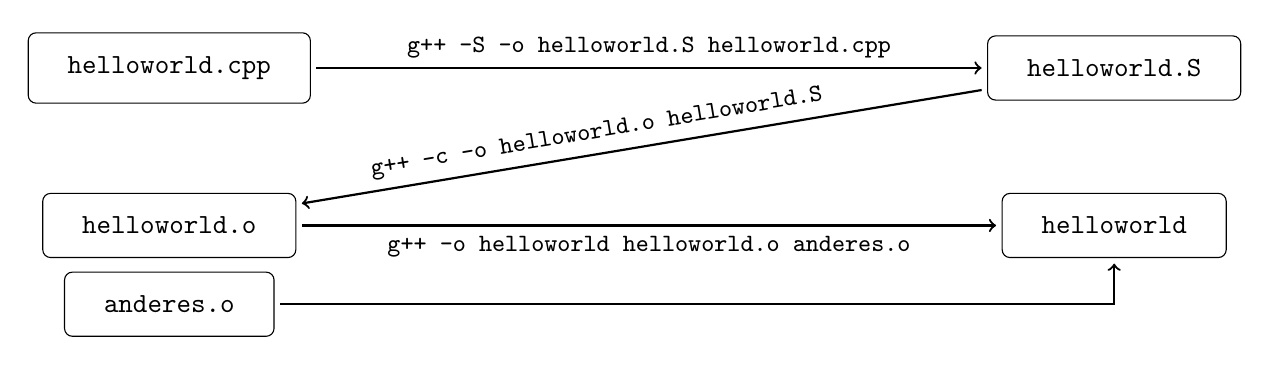
\begin{tikzpicture}
	\tikzstyle{block} = [ shape=rectangle, rounded corners = 0.1cm, draw=black, inner xsep=0.5cm, inner ysep = 0.3cm ];
	\tikzstyle{arr} = [ ->, thick, shorten >= 2pt, shorten <= 2pt ];

	\node (nHelloWorldCpp) [block] {\texttt{helloworld.cpp}};
	\node (nHelloWorldS) [block, right of = nHelloWorldCpp, node distance = 12cm] {\texttt{helloworld.S}};
	\draw [arr] (nHelloWorldCpp) -- (nHelloWorldS) node [midway,above,font=\small] {\texttt{g++ -S -o helloworld.S helloworld.cpp}};
	\node (nHelloWorldO) [block, below of = nHelloWorldCpp, node distance = 2cm] {\texttt{helloworld.o}};
	\draw [arr] (nHelloWorldS) -- (nHelloWorldO) node [pos=0.56,above,sloped,font=\small] {\texttt{g++ -c -o helloworld.o helloworld.S}};
	\node (nAnderesO) [block, below of = nHelloWorldO, node distance = 1cm] {\texttt{anderes.o}};
	\node (nHelloWorld) [block, below of = nHelloWorldS, node distance = 2cm] {\texttt{helloworld}};
	\draw [arr] (nHelloWorldO) -- (nHelloWorld) node [midway,below,font=\small] {\texttt{g++ -o helloworld helloworld.o anderes.o}};
	\draw [arr] (nAnderesO) -| (nHelloWorld) node {};
\end{tikzpicture}

Der bisherige Befehl, den wir zum Kompilieren benutzt haben, ist tatsächlich
nur ein Spezialfall von diesem: Geben wir nämlich auf der Kommandozeile eine
input-Datei an, so rät \texttt{g++} anhand der Dateierweiterung und der
Parameter, was wir damit tun wollen. Er führt dann alle Schritte, um von
unserer input-Datei zu der gewünschten zu kommen automatisch aus, wenn wir also
\texttt{g++ -o helloworld helloworld.cpp} eingeben, dann weiß der Compiler,
dass wir eine ausführbare Datei wünschen (da wir weder \texttt{-c} noch
\texttt{-S} angegeben haben) und dass er dafür preprocessen, kompilieren, assemblieren und
linken muss (da wir ihm eine \texttt{.cpp} Datei gegeben haben).
\begin{praxis}
	\begin{enumerate}
		\item \texttt{assemble.cpp} enthält ein kleines (ziemlich nutzloses)
		      Programm, welches zwei Zahlen addiert und das Ergebnis ausgibt.
		      Kompiliert es (nun nur der erste Schritt in dem Diagramm, nicht so, wie
		      in den vergangenen Lektionen) und schaut euch das resultierende
		      \texttt{.S}-file in einem Editor an. Ihr müsst nicht verstehen,
		      was genau hier überall passiert, aber vielleicht findet ihr ja die
		      \texttt{main}-Funktion, die Definition der Variablen und die Addition?

		      Wir können nun mal Optimierung anschalten -- gebt dazu zusätzlich den
		      Parameter \texttt{-O3} direkt nach dem \texttt{g++} an. Schaut euch das
		      \texttt{.S}-file nun wieder im Editor an. Was fällt euch
		      (im Vergleich zu vorher) auf?
		\item Assembliert eines der im vorigen Schritt erzeugten \texttt{.S} files
		      in ein \texttt{.o}-File.
		\item Benennt in einem eurer bisherigen Programme die
		      \texttt{main}-Funktion um und versucht, es zu kompilieren (wie in den
		      bisherigen Lektionen, also alle Schritte auf einmal). Schaut euch die
		      resultierenden Fehlermeldungen an. Wo wird euch der Linkerfehler
		      ausgegeben?
		\item Macht die Umbenennung wieder rückgängig und kompiliert das Programm
		      erneut -- übergebt aber dieses mal den Quellcode doppelt (also z.B.
		      \texttt{g++ -o helloworld helloworld.cpp helloworld.cpp}). Was
		      beobachtet ihr? Könnt ihr die Beobachtung erklären?
	\end{enumerate}

	\inputcpp{assemble.cpp}
\end{praxis}
